\documentclass[11pt]{article}

\usepackage[margin=1in]{geometry}
\usepackage{graphicx}
\usepackage{verbatim}
\usepackage{listings}
\usepackage{amsfonts}
\usepackage{textcomp}

\title{Distributed Graph Processing for Machine Learning:\\
The Case for Condor and Spot Instances}
\author{Jing Fan~~~~~Ce Zhang}
\date{}

\begin{document}
\maketitle

\begin{abstract}
We study distributed graph processing for machine learning
applications in an environment
in which the failure of workers is guaranteed to happen
frequently. Notable examples of such environments can be found
both in the classic grid computing, e.g., Condor, and the emerging
cloud computing, e.g., {\em spot instances} on Amazon EC2.
Different from the common practice that running
machine learning algorithms with a dedicated cluster,
it is still an open research question that how (and whether
it is possible) to run machine learning algorithms in
this environment.

This report documents our {\em preliminary} effort towards 
answering this question by building a prototype system. 
Ideally, we have two goals: (1) {\em expressiveness}:
this prototype system should allow the user to specify
a machine learning system as easy as existing frameworks
designed for dedicated clusters; and (2) {\em efficiency}:
the machine learning system specified by the prototype system
should be able to run in environments such as Condor efficiently.
We report our design of this prototype system that extends
the programming model of a popular graph-processing engine,
namely GraphLab. Given a user program written in our language
extension, we describe the execution model. We validate
our prototype system with an emergingly popular machine
learning application, namely deep neural network, on {\em both}
Condor and Amazon EC2. We find that our prototype system is
able to achieve more than 12TFLOPS on Condor with more than
2.6K cores harvest from the national Open Science Grid (OSG).

\end{abstract}

\section{Introduction}

Machine learning has been one emerging area that
attracts interests from the community of system 
research, especially research of 
distributed systems~\cite{Li:2014:OSDI,GraphLab:OSDI,Spark,Google,Yahoo}. 
Notable examples include GraphLab~\cite{GraphLab:OSDI},
Spark~\cite{Spark}, Google's DistBelief~\cite{Google}, and 
Yahoo's Parameter Server~\cite{Yahoo,Li:2014:OSDI}. 
In this work, we focus on the same goal, that is 
to build a framework that supports executing machine 
learning applications in a distributed environment.

It has been a common practice for distributed machine
learning systems to be run on dedicated clusters.
For example, both Spark and GraphLab have been 
reported to be able to execute machine learning algorithms
on hundreds of machines; DistBelief is able to 
train deep neural network on 6000 machines; and 
Parameter Server is able to scale to 1000 machines.
Our key observation is that existing frameworks~\cite{Li:2014:OSDI,
GraphLab:OSDI,Spark,Google,Yahoo} implicitly
make {\em at least one} of the following two assumptions
about the distributed environment and workload:

\begin{enumerate}
\item The coordinators know {\em a priori} 
the set of worker nodes, including their configuration,
number of worker nodes, and the network topology between
these workers. These information are necessary for most
existing systems to schedule their workload before
execution. For example, Yahoo's Parameter Server
uses consistent hashing~\cite{Li:2014:OSDI} to allocate
resources and workers, and use chain replication to
deal with worker failures. GraphLab~\cite{GraphLab:OSDI} also
uses similar approaches. 
\item The graph to be processed consists of nodes that are 
executed with the same level of consistency. For example,
in GraphLab, the execution engine can choose from three
different consistency levels, and all the nodes in the same
graph will follow the same level.  
\end{enumerate}

These assumptions are often true in the environment that
these systems are designed for, in which the cluster is
maintained in a centralized way or leased from cloud-based
services (e.g., EC2). However, this assumption
does not always hold for a popular environment that
often be called {\em high throughput computation} (HTC) 
environment. One notable example is Condor, which,
when ran on the national open science grid, can easily
harvest hundreds of thousands of machine hours per day.
Another example is the spot instance on Amazon EC2, which 
relies on a bidding-based model that could provide much
cheaper solution than traditional cloud-based instances.
These HTC environments have the characteristics that are
different from the above two assumptions when applied to 
machine learning.

\begin{enumerate}
\item The coordinators do not know the set of workers
{\em a priori}. For example, in Condor, the coordinator
does not know how many workers will be assigned to it, and
what type of machines will be assigned to it. Also, the
workers are not guaranteed to be able to communicate with each
other. Similar scenario applies to spot instances
of EC2, in which the number of workers assigned to the
coordinator depends on the bidding price and other bidder, while
the configuration of machines are known to the coordinator.
\item Machine learning workload often contains heterogeneous
consistency requirement. For example, for some data
in machine learning workload, full consistency is not required,
while for other data, one might need higher-level of consistency.
This observation has also been made in a subset of
existing systems, e.g., Parameter Server~\cite{Li:2014:OSDI}.
\end{enumerate}

We study how to build a GraphLab-like system with these two
observations, and study their implications on system design.
We first propose a language extension of GraphLab for the
user to specify a machine learning algorithm, and use
Deep Neural Network (DNN) as an use case. We then study
the design decisions we made for both Condor and spot
instances of Amazon EC2. We validate our prototype system
on standard benchmark data sets.

\section{System Design}

We describe the design decisions and how they relate to
the two observations we made on Condor and spot
instances of Amazon EC2. We first describe in more details
about these environment, and present the language extension
and execution model.

\begin{figure}[t]
\centering
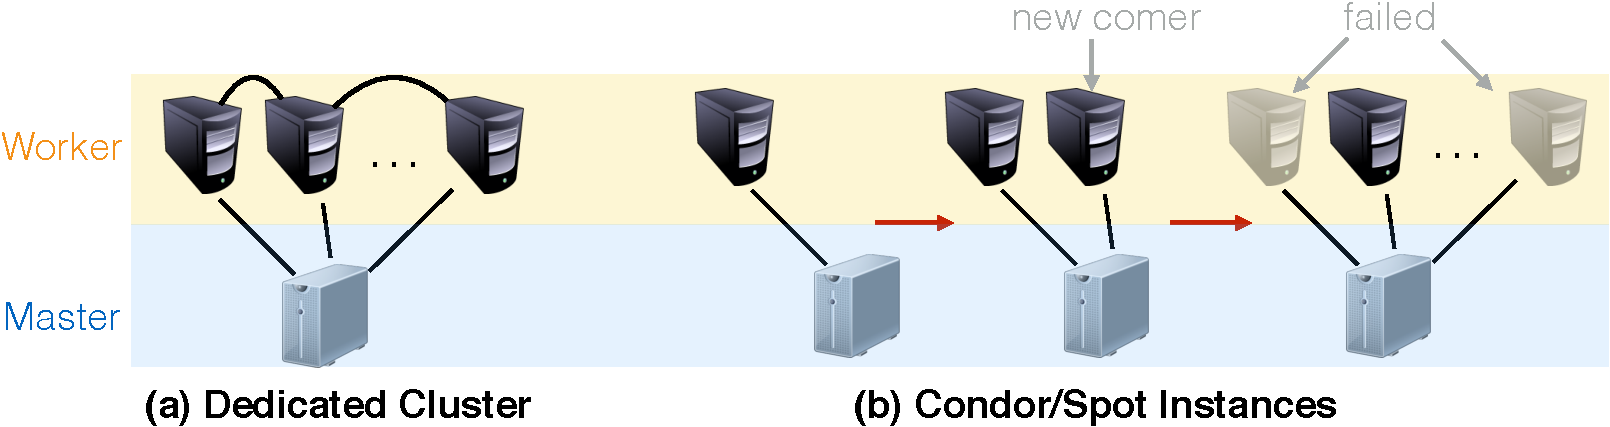
\includegraphics[width=0.9\textwidth]{figures/env-crop}
\caption{An illustration of (a) dedicated cluster and (b) Condor/Spot-instances. (b) illustrates three states in different time where the worker machines keeps come in and fail.}
\label{fig:env}
\end{figure}

\subsection{Condor and Spot Instance of EC2}

Figure~\ref{fig:env} illustrates the difference between
a dedicated cluster, Condor instances, and EC2 instances.
We describe their difference as follows.

\paragraph*{Dedicated Cluster} The dedicated cluster
that existing work assumes usually contains two components:
(1) a set of master machines; and (2) a set of worker machines.
In some frameworks, master machines and worker machines
could overlap. A dedicated cluster starts from a given
set of machines, and when the job starts, this number is
known to the system. Therefore, one could use techniques
like consistent hashing to allocate resources. Failures
are assumed for both worker and master, and therefore,
one could use techniques like chain replication. However,
the failure rate is usually low compared with the two scenario
that we are going to discuss later.

\paragraph*{Condor} Figure~\ref{fig:env}(b) illustrates
the case for Condor. Similar to dedicated cluster, there
are workers and masters. The cluster starts with only
master machines and zero workers. During execution,
workers are added to the pool periodically, but also
fail periodically. According to the statistics we get
from OSG, the same worker usually has a life span around
45 minutes, which means, after 45 minutes a worker will
exit with a large probability. Usually, workers cannot 
communicate with each other
because they are behind the firewall of different organizations
cross the country.

\paragraph*{EC2 Spot Instances} The spot instances
of EC2 has similar structure with Condor. New instances
will be added into the pool when the bidding price is
higher than the market price; and instances will be removed
from the pool when the bidding price is lower than
the market price. Because the market price is unknown and
keep changing dynamically, there is no way for the master
to know beforehand the number of worker machines.

\subsection{Language Extension}

We first describe the formal model of our language extension,
and the vertex-centric API we provide for the user to specify
machine learning algorithms as graph-processing workloads.
This language extension is motivated by the observation that
different vertices could have different requirement of consistency.

\paragraph{Language Model of GraphLab} Let $G=(V,E)$ be a graph, where 
$V$ is a set of vertex and
$E\subseteq V^2$ is a set of edges between vertices. Given a vertex $v \in V$,
%let $D_v$ be the state of $v$ that can be arbitrary type of user defined POD 
%structure, and define similarly $D_e$ for an edge $e$. Call $D$ the data, and
%let $(N_v^{(V)}, N_v^{(E)}$ be the data of vertex and edges that are neighbors 
%of $v$.\\
Let $N(v)$ be the set of neighbouring vertices with $v$. Denote the state of 
vertex $v$ in beginning of the $i$th iteration as $v^{(i)}$, and the states of 
its neigbouring vertices in the beginning of the $i$th iteration as $N(v)^{(i)}$.
In GraphLab, the user defines a function $f$ for vertex $v$ that does the 
following:
\[
 v^{(i+1)}, N(v)^{(i+1)} \leftarrow f(v^{(i)}, N(v)^{(i)})
\]

\paragraph{Extension} We propose to extend the language of GraphLab as follows. 
We first describe this extension,
and then explain the intuition behinds it.
For each vertex $v\in V$, we extend the GraphLab language with an additional 
function $agg(v)$ that does the
following: 
\[
v^{(i+1)}\leftarrow g(v^{(i)}, v'^{(i)}),
\]
where $v$ and $v'$ are 
two replicas of the same vertex. With this extension, we
could partition the graph into smaller pieces
by introducing replicas of vertex and resolve conflicts
using this aggregation function.

\subsubsection{Vertex-centric APIs}

We describe the API we provided for the user to implement
the formal model we just described.
A vertex in the graph is modeled by the \textsf{Vertex} data structure:
\begin{verbatim}
class Vertex {
  NodeIdType nodeId;
  T data;
  vector<Vertex> neighbours;
};
\end{verbatim}
We expose baisc operations of a vertex, including viewing and updating the 
value of itself and its neighbours. The APIs are shown in 
Figure~\ref{fig:api}. This API enable programmers to make queries 
from the perspective of a vertex (in a vertex-centric way). 

\begin{figure}
  \centering
  \small
 \begin{tabular}{l|l}
 \hline
 Function & Usage\\
 \hline
 NodeIdType getNodeId() & Get the id of this vertex.\\
 VertexData$\langle$T$\rangle$ getData() & Get the data of this vertex.\\
 vector$\langle$Vertex$\langle$T$\rangle$ $\rangle$\ getNeighbours() & Get all 
the neighbour information.\\
 void updateValue(NodeIdType nodeId, VertexData$\langle$T$\rangle$ val) & Update 
the value of vertex nodeId to val.\\
 \hline
 \end{tabular}
 \caption{APIs and Usage}
 \label{fig:api}
\end{figure}

\subsubsection{Example of Deep Neural Network for Image Recongnition}
We illustrate the usage of the system by the example of deep neural
network	for image recognition. In DNN, we have two kind of vertices, one 
being the vertex that stores the real image data and the other being the neural 
network vertex that contains the parameters to learn. 
We define \textsf{f.cpp} for the image vertices and \textsf{g.cpp} for the 
``averagble'' neural netowrk vertex, as shown in Listing~\ref{lst:f}~\ref{lst:g}.
\begin{lstlisting}[language=java,basicstyle={\ttfamily\small},caption={f.cpp},label={lst:f},frame=single]
 int main(){ 
   // get vertex content
   Image *img = getData<Image>();
   // get neighbors’ content 
   vector<Node> neighbours = getNeighbours(); 
   Network *nw = getData<Network>(&neighbours[0]); 
   NodeId nwId = nw.nodeId;
   // do training of neural network
   Layer *layer1 = nw->layers[0];
   Layer *layer6 = nw->layers[5];
   layer6->ops[0]->label = img->label; for (int i = 0; i < 4; ++i) {
   layer1->ops[i]->inputs[0] = img->content; }
   nw->forward();
   nw->backward();
   // write back new content 
   updateValue<Network>(nwId, nw);
 }
\end{lstlisting}
\begin{lstlisting}[language=java,basicstyle={\ttfamily\small},caption={g.cpp},label={lst:g},frame=single]
 int main(){ 
   // get two replicas 
   Network *nw1 = getData<Network>(); 
   Network *nw2 = getData<Network>();
   // do the average 
   nw1->avg_with(nw2); 
   nw2->copy_from(nw1);
   // write back new content 
   updateValue<Network>(getNodeId(), nw1);
 } 
\end{lstlisting}

\subsection{Execution Model}
The vertices have difference levels of consistency, correspondingly, we have 
different types of workers. We denote the vertices that don't have $agg$ 
function as type $A$ and otherwise type $B$. We define two kinds of workers:
\begin{itemize}
 \item \textbf{Remote workers} are responsible for type $A$ vertices. Typically we 
deploy these workers on unreliable low-end servers, such as condor servers.
 \item \textbf{Master workers} are responsible for type $B$ vertices. Typically we 
deployed these workers on reliable high-end servers.
\end{itemize}

We first decompose the graph into different connected components by introducing 
replicas for ``averagble'' vertices.
If there are no ``averagble'' vertices in the graph, we follow the BSP mode of 
GraphLab to uniformly partition the graph.
Each Condor job contains a set of vertices in the same partition.
In every iteration, the master node submits all Condor jobs.
The execution model for each type of workers is as follows:

\begin{itemize}
\item \textbf{Remote workers.} Run $f()$ for every type $A$ vertices, which reads the local copy of type $B$ 
vertices and update the local copy of type $B$ vertices. (All “updates” are 
atomic, meaning that no read operation will read a parital update.)
\item \textbf{Master workers.} For each Condor job that is running, read the remote copy of type $B$ vertices, 
run $g()$ to average with local copy, and \texttt{scp} it to the running Condor job. 
This step happens in an asynchronized way. For each finished Condor job, reads 
its final state of type $B$ vertices, run $g()$ to average with the local copy 
and update the local copy.
\end{itemize}

\paragraph*{Deciding the Chunk Size}

One key parameter that we need to decide is the
chunk size, that is the number of vertices we
put in a single Condor job. We develop the following
analytic model to estimate this parameter. 

Let $N$ be the total number of vertex, and $t_{exec}$
be the time that a single vertex needs to
finish execution. Let $t_s$ and $t_e$ be the time
that Condor needs to start and end a job. Let
$t_c$ be the time that each vertex requires to copy
to the worker.
Let $T$ be the time that a Condor worker can execute
before getting killed. Let $n$ be the number of 
vertex we put in a single Condor job.
%
We have that there are $N/n$ Condor jobs, each of which
takes $nt_{exec}$ time to execute. 

\subparagraph*{Infinite Bandwidth with Deterministic Failure}

We assume that the master has infinite bandwidth (which
is usually the case for computationally expensive
workload such as DNN),
and therefore, no matter how many jobs we have, they
do not interfere with each other. In this case, the
total execution time is
\[
TotalTime(n) = \frac{N}{n} \mathbb{I}_{T>n(t_c+t_{exec})} \left[ t_s + nt_c + nt_{exec}  + t_e \right]
\]
If we want to maximize
\[
\frac{Nt_{exec}}{TotalTime(n)}
\]
we just need to set
\[
T=n(t_c+t_{exec}).
\]

\subparagraph*{Infinite Bandwidth with Stochastic Failure}

Our previous analysis assumes that Condor jobs fail
deterministically after time $T$. A more tight and realistic
analysis is to assume this parameter is stochastic. For example,
let $T\sim\mathcal{N}(\mu, \sigma^2)$ be a Gaussian random variable.
Now $TotalTime(n)$ becomes a random variable.
Instead of analyzing this random variable as a whole, let's
look at a single job.
\[
TimeOfAJob(n) = \mathbb{I}_{T>n(t_c+t_{exec})} \left[ t_s + nt_c + nt_{exec}  + t_e \right]
\]
The expectation of this random variable is
\[
\mathbb{E}\left[TimeOfAJob(n)\right] = \Pr[T>n(t_c+t_{exec})] \left[ t_s + nt_c + nt_{exec}  + t_e \right]
\]
Let $\Phi_{\mu,\sigma}$ be the quantile function
of the Gaussian distribution, we have
\[
\mathbb{E}\left[TimeOfAJob(n)\right] = \Phi(n(t_c+t_{exec})) \left[ t_s + nt_c + nt_{exec}  + t_e \right]
\]
Trivially, the expectation of $TotalTime(n)$ becomes
\[
\mathbb{E}\left[TotalTime(n)\right] = \frac{N}{n} \Phi(n(t_c+t_{exec})) \left[ t_s + nt_c + nt_{exec}  + t_e \right]
\]
The best chunk size should be the one that minimizes this 
expectation. However, it is well-known that the quantile
function of Gaussian cannot be expressed in closed form in 
terms of elementary functions; therefore, one can use
standard numerical methods to search for (local) minimal
of this function.


\paragraph*{Extension to Spot Instances of EC2}

We describe how our design could be extended to spot instances
on EC2 easily, with a few twists. Compared with a Condor-based
environment, spot instances lack the ability to automatically
schedule a job (e.g., copy data, execute, and copy data back
to master). Therefore, we twist our Condor-based implementation
in the following ways.
\begin{enumerate}
\item {\bf Default AMI.} We create a user-defined AMI that contains
the following routine: (1) When the AMI starts, it starts a daemon
that pings the master IP, which is stored in the AMI; (2) it
automatically downloads a chunk of jobs from an address provided
by the master; (3) it starts execution of a binary that is
already in the AMI; (4) it copies results back when finished
or evicted.
\item {\bf Master Worker.} The master worker has a simple twist
that it manages the copy of jobs to the remote worker by itself
by passing the local path name to enable \texttt{scp} from 
the remote worker. 
\end{enumerate}

We implement this strategy and uses \$0.1 to bid 100 c1.xlarge
instance that has 4 virtual CPU. We report the performance in 
Section~\ref{sec:perf}.


\section{Performance Study} \label{sec:perf}

We describe experiments that validate the performance of our systems.
We first describe the end-to-end experiments, and then two
experiments about choosing chunk size and executing jobs on EC2.

\begin{figure}[t]
\centering
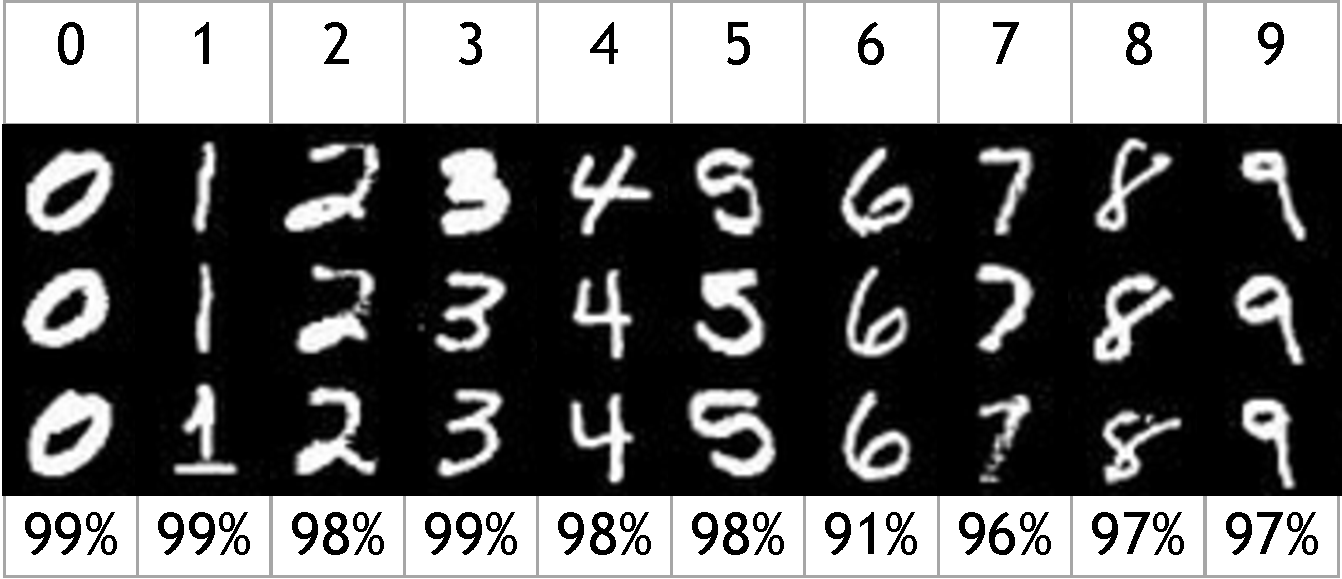
\includegraphics[width=0.5\textwidth]{figures/result-crop}
\caption{An Illustration of the MNIST datasets with
example predictions and accuracy of our prototype system.}
\label{fig:mnist}
\end{figure}


\subsection{End-to-end Experiment}

We validate that our prototype system is able to conduct
learning of Deep Neural Network on standard benchmark dataset
efficiently.

\paragraph*{Data Sets} We conduct experiment on two standard
benchmark datasets, namely ImageNet and MNIST. MNIST is the
{\em de facto} benchmark of handwriting recognition that contains
60K 28$\times$28 images illustrated as in Figure~\ref{fig:mnist}. ImageNet
focuses on image recognition and is one of the largest corpus
that contains 1.8M images. After following state-of-the-art to
resize the images in ImageSize into 224$\times$224, the whole
corpus is 46GB.

\paragraph*{Protocol} We execute the DNN application with the
code we described in previous sections. We select the chunk size with
our analytic model with deterministic failure. The master
machine has two 6-core 2.4GHz Xeon CPUs and 128GB RAM.
We record the time for one training epoch of both corpus
and also calculate the number of floating point operations
we can do per second (FLOPS). Because existing framework
cannot be installed on Condor, it is hard to compare with them.
Therefore, we compare our system with a single-GPU implementation
with Nvidia Titan, one of the toppest GPUs available on the market.

\paragraph*{Result} Our run on ImageNet finishes a single
iteration in 0.87 hours. Compared with the execution time of
GPU, we are 3.1$\times$ faster. At peak time, we harvest
2.6K cores on Condor, and around 12T FLOPS. It is not surprising
that our distributed implementation is only 3 times faster
than a single GPU for two reasons. First, a single GPU contains
more than 2000 computation units, and therefore is of roughly
the same size as the number of cores we harvest on Condor.
Second, many machines on Condor are relatively old, and only 12\%
of the machines we harvested support AVX. For machines that
AVX is not supported, we can only do less than 4 single-precision
floating point operations per CPU cycle.


\begin{figure}[t]
\centering
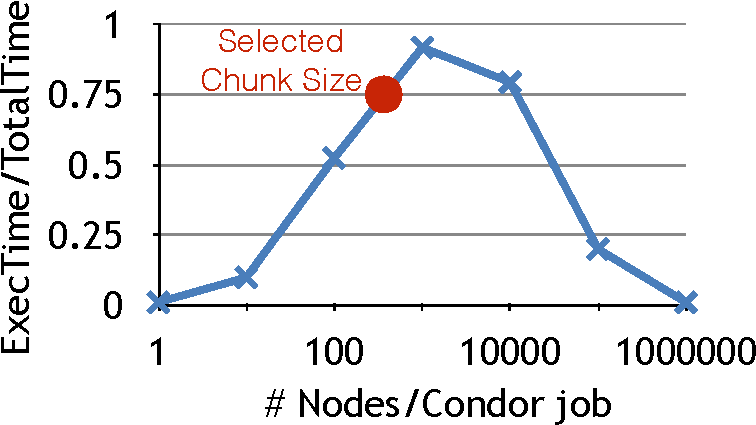
\includegraphics[width=0.4\textwidth]{figures/chunk-crop}
\caption{The Selection of Chunk Sizes.}
\label{fig:chunksize}
\end{figure}


\subsection{Chunk Size Selection}

We validate that our analytic model for chunk size selection
achieves a near optimal selection. We use our deterministic
failure model, and vary the number of nodes per Condor job.
To conduct the experiment, we replicate the MNIST datasets
to create 1M jobs. We plot the ratio of execution
time and total execution time in Figure~\ref{fig:chunksize}.

From Figure~\ref{fig:chunksize} we see that, consistent
with our expectation, there exists an optimal chunk size
when we vary the chunk size. The choice of a suboptimal
chunk size could be catastrophic and can be up to
two orders of magnitude less efficient than the optimal choice.
Our analytic model is able to select a near optimal
chunk size, which is within 25\% of the efficiency of 
the optimal choice.

\subsection{Running on Amazon EC2}

We report our preliminary result of running our prototype
system on Amazon EC2. We bid 100 c1.xlarge instances with 
the price of \$0.1. Each c1.xlarge instance has
4 virtual CPU, and we also find that AVX2 is supported, and
therefore, the peak performance is 16 floating point
operation per cycle for fused \texttt{MULPS} and \texttt{ADDPS} instructions.
Our bided price is too high such that all 100 instances
keep running for one hour. This gives us 4.5T FLOPS.
Because we cost \$0.002 per second, this is 2250T FLOPS/\$.

We hoped to lower the price and expect this will give us
more interesting result. However, any sanely designed
experiments in our mind would take more than \$100. Therefore,
we did not conduct these experiments.

\bibliographystyle{abbrv}
\bibliography{report}

\end{document}


















